\chapter[Resultados]{Resultados}

A partir do estudo e pesquisa realizado até o momento determinamos o que utilizar no conjunto do sistema, levantando um perfil que a equipe acredita ser a mais viável em termos de interação, custo-benefício, tempo, conhecimento técnico e outros fatores importantes para o projeto. Será desenvolvido um kit com capacidade de ser acoplado em diversas cadeiras de rodas afim de facilitar a mobilidade elétrica em cadeiras manuais. Os resultados levantados estão disposto logo abaixo.

\section{Estrutura}

Com a utilização do programa CATIA V5 3D foi estruturado o sistema eletrônico acoplado à cadeira de rodas, \ref{fig:frontal}. Visando três preceitos básicos: comodidade, acessibilidade e conforto.

\begin{figure}[!htb]
\centering
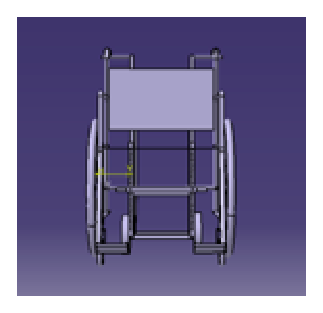
\includegraphics[keepaspectratio=true,scale=0.4]{figuras/estrutura/vista_frontal}
\caption{Vista Frontal}
\label{fig:frontal}
\end{figure}

O objetivo do projeto é desenvolver uma estrutura de fácil conexão e resistente. O produto proposto, ver figura \ref{fig:traseira},\ref{fig:sistema}, \ref{fig:lateral} e \ref{fig:superior},deve-se acoplar a qualquer cadeira de rodas. Foi pensado em um dispositivo no formato de uma mala para que seja de fácil conexão, uso e manuseio.

\begin{figure}[!htb]
\centering
\includegraphics[keepaspectratio=true,scale=0.4]{figuras/estrutura/vista_traseira}
\caption{Vista Traseira}
\label{fig:traseira}
\end{figure}

\begin{figure}[!htb]
\centering
\includegraphics[keepaspectratio=true,scale=0.4]{figuras/estrutura/explode}
\caption{Visão do Sistema}
\label{fig:sistema}
\end{figure}

\begin{figure}[!htb]
\centering
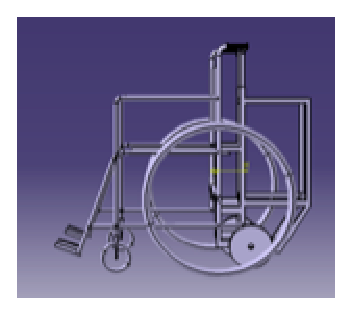
\includegraphics[keepaspectratio=true,scale=0.4]{figuras/estrutura/vista_lateral_cadeira}
\caption{Imagem Lateral}
\label{fig:lateral}
\end{figure}

\begin{figure}[!htb]
\centering
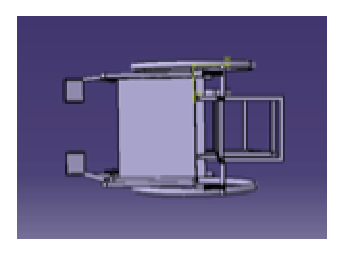
\includegraphics[keepaspectratio=true,scale=0.4]{figuras/estrutura/vista_superior}
\caption{Imagem Superior}
\label{fig:superior}
\end{figure}

\section{Power Train}
O Power Train é o conjunto de sistemas que realizam o trabalho e junção das engenharias do projeto, temos bateria, motor elétrico, sistema eletrônico, logística das rodas e torque, organização e ergonomia do projeto. Em cada item foi feito um estudo levando em conta custo-benefício das peças em questão. No kit da cadeira de rodas é utilizado motor corrente continua e baterias automotivas pela facilidade da compra e da recarga. O motor é a principal desse sistema, há diferentes tipos de motor, e o utilizado será de corrente continua capaz de suprir uma potencia necessária para o funcionamento. O sistema eletrônico será essencial com o uso da ponte “H” e aplicativos no kit integrado.

\subsection{Motor}

Será utilizado no projeto o motor de corrente contínua. A escolha foi feita pois esse tipo de motor é muito utilizado em projetos que necessitam de velocidades variáveis, eles também apresentam uma região de torque e potência constante e são simples de realizar a aceleração e a desaceleração \cite{manual_bateria_unipower}.

Especificações a serem atendidas:
\begin{itemize}
 \item Velocidade máxima de 7,2 km/h apx: 2m/s;
 \item Peso máximo de 120 kg;
 \item Peso da bateria 10 kg;
 \item Peso da cadeira (valor aproximado) 20kg;
 \item Peso total estimado: 150 Kg;
 \item Considerando hipoteticamente o coeficiente de atrito ($\mu$): 0,2.
\end{itemize}

\textbf{Força de atrito:}
\begin{equation}
 \overrightarrow{F} = \overrightarrow{N} * \mu = 150 * 9,8 * 0,2 = 294N
\end{equation}

\textbf{Potência do motor:}

\begin{equation}
 P_{x} = \frac{F * v}{100} = \frac{294 * 2}{1000} = \frac{588}{100} = 0,588kW
\end{equation}

O motor para a utilização na aplicação deve seguir algumas características dentro das especificações do projeto. Serão utilizados dois motores para motorizar a cadeira de rodas. Com isso é necessário que cada motor tenha a potência mínima de: \textbf{294W}.

\subsection{Baterias}
A bateria de chumbo-ácido é muito utilizada hoje em dia em diferentes áreas,  como automóveis, sistemas de fornecimento de energia elétrica ininterrupta (no-breaks) e cadeiras de rodas elétricas. Desprezando-se o problema do peso e considerando as observações feitas anteriormente no capítulo \ref{cap:fundamentacao_teorica} foi a bateria escolhida para o projeto, considerando ainda o seu fácil acesso e baixo  custo.

\section{Controle}

O kit de automação para cadeiras de roda será e um produto projetado para auxiliar na locomoção do cadeirante em um shopping. Na Figura \ref{fig:diagrama_blocos} foi feita uma proposta de construção do kit mostrando a sua estrutura de controle. Em verde claro tem-se um componente que talvez seja somente integrado ao sistema. Esses blocos foram resultado dos estudos teóricos e de discursões da equipe. Em verde escuro, sistemas que serão efetivamente projetados e construídos e em azul, componentes que não serão construídos mas farão parte do kit de automação.

\begin{figure}[!htb]
\centering
  \includegraphics[keepaspectratio=true,scale=0.6]{figuras/controle/diagrama_blocos}
\caption{Desenho do diagrama de blocos do sistema de controle}
\label{fig:diagrama_blocos}
\end{figure}


Para o kit de automação da cadeira de rodas, será utilizada a ponte H para o controle dos motores. Um algoritmo de controle PWM usando o Raspeberry Pi que deve responder aos comandos do usuário como direção, aceleração, frenagem, entre outros que serão posteriormente levantados. Na figura \ref{fig:diagrama_blocos} pode ser obervado o esquemático geral do sistema. Tem-se ainda o Distribuidor, uma placa para facilitar a alimentação do sistema, e o Regulador, para alimentar o Controlador e periféricos.

Será incluído ainda um sistema de segurança, para evitar que o dispositivo saia do controle do estabelecimento, esse ainda precisa ser melhor discutido para estabelecer a tecnologia que será utilizada.

O sistema vai ser projetado de forma que não seja necessário retirar a bateria para essa ser carregada, o grupo ainda não estabeleceu se o carregador vai ser construído ou comprado, considerando que o tempo disponível para o desenvolvimento do projeto é relativamente curto.

O Distribuidor vai ser basicamente uma placa que facilitara a conexão de todas as outras ao sistema, assim não será necessário que haja reduções de tensão tão drásticas. A placa terá um circuito de proteção, para evitar problemas de sobretensão e curto, saídas para a ponte H, tanto para alimentar possíveis circuitos e motor e ainda saídas para o regulador.

O Regulador terá a funcionalidade de alimentar o controlador com seus periféricos. Essa placa terá um circuito de proteção, para o controlador, contra possíveis problemas do distribuidor, saídas de alimentação para o controlador e ainda uma USB de alimentação para o celular do usuário, para impedir problemas de falta de bateria.

A ponte H será o circuito responsável por fazer o controle de velocidade e direção dos motores. Essa placa terá além dos circuitos necessários para o funcionamento da ponte H, um circuito de proteção para os motores e pinos de entrada do PWM, já que pode haver possíveis problemas de sobretensão a alimentação do motor.

Uma das linguagens que será adotada é o Python devido a facilidade de existir bibliotecas específicas que controlam o GPIO  (General Purpose  Input/Output) do Raspberry Pi. Essa linguagem é uma linguagem de programação de alto nível, interpretada, orientada a objetos, de tipagem dinâmica. Tem uma sintaxe concisa e clara, juntamente com bibliotecas com recursos poderosos. Os módulos e frameworks ainda não foram decididos.







\section{Interface com o usuário}


\subsection{Joystick}
Para as cadeiras de rodas automatizadas essa é uma solução comum de controle para as mesmas, tendo em vista que é relativamente simples de ser acoplado uma vez que se entenda seu funcionamento básico.

Para o projeto em questão essa foi uma das alternativas encontradas. No qual o joystick seria acoplado ao braço da cadeira, ou em uma posição que o usuário se sinta mais ergonomicamente confortável. Este acoplamento deve ser simples para favorecer a característica de portabilidade do projeto como um todo.

Caso necessário a conexão do joystick ao sistema de controle pode ser feita por bluetooth, tal característica contribui para o objetivo final do projeto \cite{artigo_joystick_controller}.

\subsubsection{Smartphone}
O \textit{smartphone} é um telefone celular com um sistema operacional móvel avançado que combina as características de um sistema operacional de computador pessoal com outros recursos úteis para uso móvel ou portátil \cite{article_smartphone}.

Devido a portabilidade destes dispositivos e sua facilidade de integração com outros sistemas, uma possível solução para a interação do usuário com o sistema pode ser feita. Uma conexão entre o dispositivo e o sistema será feita através de Bluetooth (Android) ou "Virtual Private Network" (iOS e Android).

Para o projeto em questão o usuário pode optar por utilizar o \textit{Smartphone} ou ainda o joystick.

\subsubsection{Protótipo}

  \begin{figure}[!htb]
		\centering
		\legend{}
    \subfloat{
  		\includegraphics[keepaspectratio=true,scale=0.6]{figuras/controle/tela_1}
		}
		\quad %espaco separador
		\subfloat{
  		\includegraphics[keepaspectratio=true,scale=0.6]{figuras/controle/tela_2}
		}
		\subfloat{
  		\includegraphics[keepaspectratio=true,scale=0.6]{figuras/controle/tela_3}
		}
		\quad %espaco separador
		\subfloat{
  		\includegraphics[keepaspectratio=true,scale=0.6]{figuras/controle/tela_4}
		}
		\caption{Protótipo de aplicativo para interface entre usuário e motor}
		\label{fig:prototipos}
  \end{figure}

O protótipo na figura \ref{fig:prototipos} foi feito com o intuito de mostrar o fluxo do aplicativo sugerido para o controle da cadeira de rodas automatizada.

A principal funcionalidade deste aplicação é basicamente voltada para o controle da cadeira de rodas automatizada, no qual o usuário teria um \textit{joystick} virtual que se comunica com o \textit{Raspeberry Pi} enviando o comando para os motores.
Uma das restrições pensadas, foi a de enquanto o controle estiver ativado via aplicativo o usuário não poderia ter o controle através do \textit{joystick} físico.

\begin{comment}
  \subsection{Controladores de potência}

  Os motores de corrente contínua utilizam das forças eletromagnéticas para transformar energia elétrica em mecânica funciona com fontes retificadas, ou seja, que possuem polaridade fixa. Esse tipo de motor, possui dois terminais, um positivo e outro negativo que de acordo com o polaridade e o sentido da corrente controlam a repulsão dos eletroímãs e consequentemente o sentido da rotação do motor.

  Uma das maiores vantagens dos motores de corrente contínua é o controle da velocidade que é feito com o dreno de corrente para o motor. Porém são mais difíceis de serem construídos e mais propícios a problemas, gerando uma maior manutenção, além disso, são propícios a problemas com faíscas internas, o que impede o seu uso em ambientes perigosos.

  Geralmente, motores precisam de correntes relativamente altas para controlar o seu funcionamento, assim é necessário que o sistema seja capaz de drenar corrente suficiente para os dispositivos. Considerando a característica dos motores de corrente contínua, sua direção é controlada pelo sentido da corrente, pode-se construir um sistema para o controle do sentido de forma simples utilizando apenas chaves. Na figura \ref{fig:direcionamento_motores} tem-se o funcionamento dos motores de acordo com a combinação das chaves indicando que o seu sentido é proporcional ao da corrente.

  \begin{figure}[!htb]
  \centering
    \includegraphics[keepaspectratio=true,scale=0.6]{figuras/controle/direcionamento_motores}
  \caption{Direcionamento dos motores}
  \label{fig:direcionamento_motores}
  \end{figure}

  O controle feito por chaves é relativamente efetivo, barato e simples, contudo, essas facilidades podem causar alguns problemas. Por se tratar de um sistema físico, a chave, com o tempo, sofre desgaste físico e está propícia a problemas estruturais e até mesmo de acionamento por sistemas automatizados. Tem-se ainda a trepidação durante um acionamento que pode acabar gerando falsos positivos. Uma alternativa para esses problemas são os transistores operando no lugar das chaves.

  O acionamento dos transistores é feito de forma elétrica, não possuindo assim desgaste físico e podem ser feitos usando baixas tensões ou correntes, o que torna o sistema mais simples. Considerando que esse tipo de componente pode atuar como porta lógica, é possível trabalhar com mais estados e uma margem maior para as necessidades do sistema. Outra vantagem é que existem vários tipos de transistores com diferentes características que podem ser agregadas ao projeto para funcionalidades como a proteção dos pinos, entre outros.

  O uso de transistores como chaves permite que sejam criados sistemas mais complexos que permitem estados diferentes, como manter o motor parado. Um circuito geralmente utilizado para esse tipo de controle é a ponte H, que é basicamente um conjunto com alguns transistores construídos de modo que a corrente possa ser direcionada de acordo com a necessidade do sistema, como pode ser visto na figura \ref{fig:motor_ponte_h}.

  \begin{figure}[!htb]
  \centering
    \includegraphics[keepaspectratio=true,scale=0.6]{figuras/controle/motor_ponte_h}
  \caption{Circuito com ponte H}
  \label{fig:motor_ponte_h}
  \end{figure}

  O transistor usado na figura \ref{fig:motor_ponte_h} é um transistor bipolar, que possui materiais polarizados e junções coladas, devido às suas características, não funciona muito bem em sistemas de potência, dificultando o seu uso para motores que drenam muita corrente. Para aplicações que exigem a passagem de corrente, são utilizados os transistores de efeito de campo, FET, que suportam mais corrente devido à sua alta impedância de entrada. Como o próprio nome diz, esse tipo de transistor é acionado com um campo elétrico na porta \textit{Gate}. Devido a esse comportamento o acionamento fica praticamente isolado, o que permite uma maior passagem de corrente com uma proteção maior para os pinos de controle.

  O acionamento dos transistores é feito a partir de uma onda quadrada, o PWM (\textit{Pulse Width Modulation}). O PWM é basicamente um onda com vários pulsos que possuem a sua largura controlada, figura \ref{fig:ondas_quadradas}, que é chamado de \textit{Duty Cycle}, essa largura determina o tempo com o qual os transistores ficarão ligados, controlando assim a passagem de corrente e a velocidade dos motores.

  \begin{figure}[!htb]
  \centering
    \includegraphics[keepaspectratio=true,scale=0.5]{figuras/controle/ondas_quadradas}
  \caption{Duty Cycle}
  \label{fig:ondas_quadradas}
  \end{figure}

  Para o kit de automação da cadeira de rodas, como uma primeira visão, será utilizada a ponte H para controle dos motores. Um algoritmo de controle PWM usando o Raspeberry Pi que deve responder aos comandos do usuário como direção, aceleração, frenagem, entre outros que serão posteriormente levantados. Na figura \ref{fig:esquema_controle} pode ser obervado o esquemático geral do sistema. Tem-se ainda o Distribuidor, uma placa para facilitar a alimentação do sistema, e o Regulador, para alimentar o Controlador e periféricos.

  \begin{figure}[!htb]
  \centering
    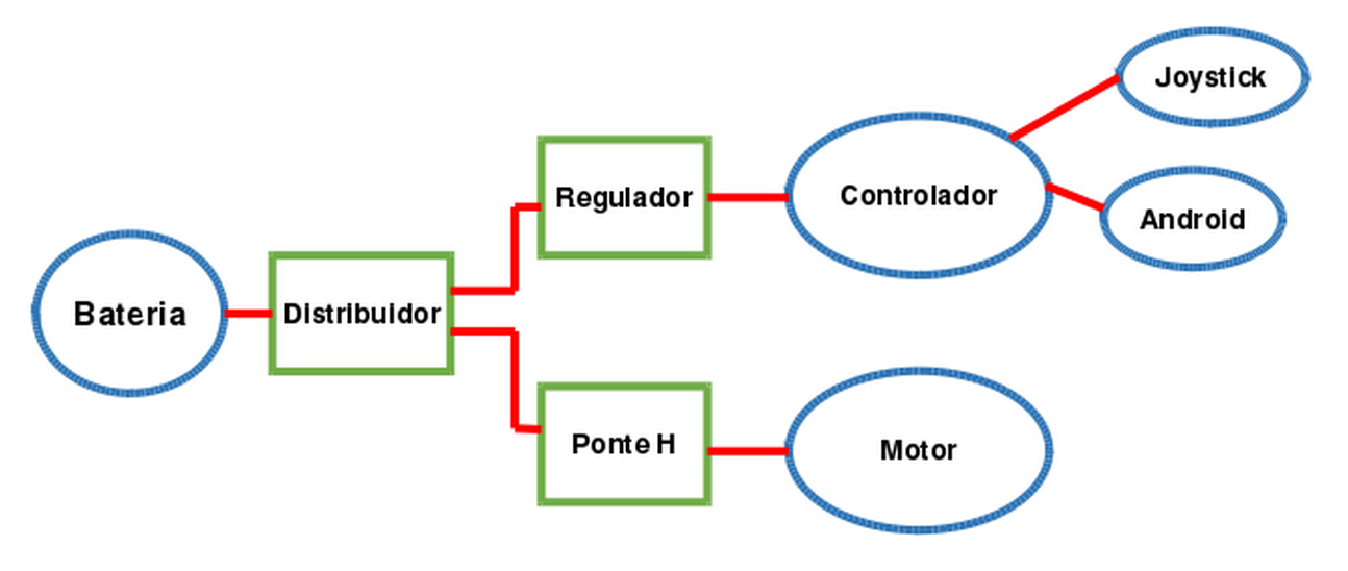
\includegraphics[keepaspectratio=true,scale=0.6]{figuras/controle/esquema_controle}
  \caption{Esquemático geral do sistema}
  \label{fig:esquema_controle}
  \end{figure}

\end{comment}

\subsection{Tecnologias}

\subsubsection{Raspeberry Pi}

É um pequeno computador que será responsável pelo controle do motor, seu modelo ainda será decidido. A escolha foi feita devido ao número de recursos oferecidos e o baixo custo desse componente.

O Raspberry Pi tem como principal componente um pequeno circuito integrado que reúne o processador com a arquitetura ARM, a GPU VideoCore IV e a memória RAM que é compativel com o sistema operacional GNU/Linux. As especificações gerais do modelo mais provável a ser utilizado no projeto, o \textit{Raspberry Pi Model B}, que pode ser visto na figura \ref{fig:rasp}, são:

\begin{itemize}
 \item Processador ARM 11 de 700 MHz;
 \item GPU VideoCore IV de 250 MHz;
 \item 256 MB total de RAM;
 \item Saída de vídeo HDMI e RCA;
 \item Saída de áudio P2;
 \item Interface de rede Ethernet;
 \item 2 portas USB;
 \item Conector Micro USB para alimentação (5 volts, 700mA).
\end{itemize}

\begin{figure}[!htb]
\centering
  \includegraphics[keepaspectratio=true,scale=0.6]{figuras/controle/blueprint_rasp}
\caption{Esquemático componentes Raspeberry Pi}
\label{fig:rasp}
\end{figure}

\subsubsection{Linguagem de programação}

Uma das linguagens a ser adotada será o Python devido a facilidade de existir bibliotecas específicas que controlam o GPIO (General Purpose Input/Output) do Raspberry Pi.

Essa linguagem é uma linguagem de programação de alto nível, interpretada, orientada a objetos, de tipagem dinâmica. Tem uma sintaxe consisa e clara, juntamente com bibliotecas com recursos poderosos. Os módulos e frameworks ainda não foram decididos.
